% !TEX TS-program = pdflatex
% !TEX encoding = UTF-8 Unicode
% arara: pdflatex: { draft: true }
% arara: biber
% arara: pdflatex: { synctex: true }
% arara: pdflatex: { synctex: true }

\documentclass[11pt]{article}
\setcounter{secnumdepth}{5}
\setcounter{tocdepth}{5}
\usepackage{float}
\restylefloat{table}
\usepackage[swedish]{babel} % Enables swedish typesetting, needs to be at top of document
\usepackage[T1]{fontenc}
\usepackage[utf8]{inputenc} % set input encoding (not needed with XeLaTeX
\usepackage{textcomp} % Suppress unicode char error
\usepackage{enumitem} % resume numbering in enumerations
\usepackage[bottom = 110pt]{geometry} % to change the page dimensions
%\geometry{a4paper} % paper format, could also be placed in documentclass options
\usepackage{graphicx} % support the \includegraphics command and options
\usepackage[parfill]{parskip} % Begin paragraphs with an empty line rather than an indent
\usepackage{verbatim} % adds environment for commenting out blocks of text & for better verbatim
%\usepackage{titling} % required for setlength droptitle (below)
%\setlength{\droptitle}{-70pt} % Adjust title height
\usepackage{fancyhdr} % This should be set AFTER setting up the page geometry
\pagestyle{fancy} % options: empty , plain , fancy
%\renewcommand{\headrulewidth}{0pt} % customise the layout...
%\lhead{}\chead{}\rhead{} % fancyhdr style reset for header
\usepackage{fancyvrb}
%\lfoot{}\cfoot{\thepage}\rfoot{} % fancyhdr style reset for footer
%\usepackage{sectsty} % Section title
\usepackage{hyperref} % href
\usepackage{caption}
\usepackage{subcaption}
\usepackage{nameref} % Enable referring to the actual name of the chapter
\usepackage[style=authoryear,backend=biber,maxcitenames=1]{biblatex}
\renewcommand*{\labelnamepunct}{\addcolon\space}
\bibliography{references.bib}
\usepackage{url}

\title{Mobile-first eller Desktop-first, en studie om utvecklingslösningar för den responsiva webben}
\author{Eduardo Castaneda}
%\date{} % Uncomment to hide date, or provide a date to display


\pagestyle{fancy}               % Fräcka sidhuvuden
\addtolength{\headwidth}{0cm}   % Sidhuvd bredare än texten.
\renewcommand{\headrulewidth}{0.4pt}
\renewcommand{\footrulewidth}{0.4pt}

\begin{document}

\maketitle
\thispagestyle{empty}


\newpage

\begin{abstract}
Abstract goes here... Lorem ipsum dolor sit amet, consectetur adipiscing elit. Nam sollicitudin varius libero ac consectetur. Nullam ornare, massa et sagittis consectetur, neque mi scelerisque arcu, in fringilla lectus risus non arcu. Suspendisse vestibulum tellus id mauris lacinia non hendrerit nibh tempor. Proin tempor interdum justo et elementum. Ut ultricies adipiscing ipsum et pharetra. Vestibulum pretium luctus est, quis egestas augue luctus et. Praesent volutpat pharetra lectus vitae elementum.

Integer fringilla ligula eu sem semper tincidunt. Nullam mi lacus, blandit non sollicitudin eget, tempor eu ante. Cum sociis natoque penatibus et magnis dis parturient montes, nascetur ridiculus mus. Morbi ornare sem et purus consequat ac adipiscing nunc tincidunt. Curabitur nisi ante, ornare vel adipiscing et, scelerisque vitae erat. Etiam blandit egestas magna, quis dapibus nulla euismod quis. Sed interdum interdum malesuada. Suspendisse lacinia imperdiet laoreet. Maecenas ullamcorper laoreet nunc ac egestas. Cras consequat elit eu lacus sollicitudin ut pharetra magna venenatis. Suspendisse scelerisque condimentum pulvinar. Mauris ut tellus sit amet nulla porttitor tristique. Suspendisse eleifend erat sed nisi lacinia eu lacinia metus porta. Nulla pretium, risus eget semper laoreet, dolor odio malesuada eros, at mattis enim turpis gravida felis. Aliquam adipiscing varius nibh, ac auctor eros bibendum non.
\end{abstract}
\thispagestyle{empty}

\newpage
\tableofcontents

\newpage


\section{Inledning}
Användningen av mobilt internet ökar för varje dag och nya webblösningar har krävts för att nå ut till mobilanvändarna. En lösning har varit responsiva webbsidor, vilket innebär att samma webbsida rendereras olika beroende på enheten webbsidan ses ifrån. Tekniken för att skapa responsiva webbsidor existerar, med hjälp av utvecklingen av tekniker och verktyg så som CSS, HTML finns i nuläget möjligheten att skapa webbsidor som beroende på skärmstorlek har olika designlayouts med en och samma kodgrund. Det finns även kunskap om hur man skall gå tillväga för att skapa en responsiv webbsida, där utvecklare med formler och riktlinjer kan lära sig att använda grundprinciperna fluid grid, fluid images och media queries på bästa sätt. Men vägen till att skapa en responsiv webbsida är olika.  I bloggar och forum på webben diskuteras flitigt valet av utvecklingsmetod när det kommer till responsiva webbplatser och innan implementeringen av en webbsida är detta en fråga som med stor sannolikhet dyker upp hos webbutvecklare. Utvecklingsmetoderna man diskuterar är \textit{Mobile-first} och \textit{Desktop-first}. Mobile-first och Desktop-first är två olika metoder där det responsiva angreppssättet används. Båda strävar efter samma mål men skiljer sig i prioriteringen av vilken enhet webbsidan skall vara anpassad för först.

\subsection{Mobile-first eller Desktop-first}
Det som kännetecknar metoderna är  grunden på strukturen och designen,  där storleken på webbläsaren avgör på vilket sätt den  skall ändras för att anpassas för en annan enhet. Kunskapen om metoderna var för sig har med tiden blivit större i samband med utvecklingen av responsive web design. Däremot ställs webbutvecklare kring frågan om vilken metod som appliceras bäst till den typen av webbsida som skall skapas. I dagsläget finns ingen kunskap om hur bra metoderna appliceras i jämförelse med varandra. Det finns tankar och spekulationer, därefter väljs metod utifrån dessa, komplikationer hanteras men dokumenteras inte och till slut har man en fungerande responsiv webbsida. Eftersom webbsidan är färdig implementerad finns ingen anledning till att implementera om en fungerande lösning med en annan metod, därav finns ingen större kunskap om jämförelse av implementationen med respektive metod riktat mot ett och samma resultat.

Användning av mobilt internet ökar och användningen av internet via en dator kommer med stor sannolikhet bestå. Vilket gör att en grund för val av metod är högst passande, då det redan nu och i framtiden kommer att kräva mer kunskap än vad som idag kan erbjudas från bloggar. Båda metoder har sina fördelar samt nackdelar, vilket bör lyftas fram tydligare. Även frågan som bör ställas är när dessa går att utnyttjas på bästa sätt, och kan beslutet av val leda till positiva faktorer vilka motsatta metod inte hade kunnat uppnå inom en specifik situation.

\subsection{Syfte}
Syftet med arbetet är att kunna hitta riktlinjer till när en specifik metod appliceras bäst. Det vill säga beroende på faktorer kring webbsidan hitta den metod som tillför det mest optimala lösningen för implementationen av webbsidan. Att hitta en metod som fungerar bäst i alla lägen är inte nödvändigtvis målet med arbetet då det existera många olika vinklar, vilka gör det svårt att hitta en specifik metod som ger det optimala resultatet oberoende på situation.

\vspace{0.5cm}
Frågeställningar som besvaras i rapporten är:
\begin{enumerate}
	\item I vilka lägen appliceras metoderna bäst?
	\item Vad är för- och nackdelarna med Mobile-first?
	\item Vad är för- och nackdelarna med Desktop-first?
\end{enumerate}
\vspace{0.5cm}
\textit{Frågeställning 1} baseras på miljö, målgrupp och kontext. Syftet med frågeställningen är att kunna utifrån analys hitta situationer där metoderna visar sig vara fördelaktiga under utvecklingsfasen, för att hitta faktorer hos metoden vilka motsatta metod inte har och därmed inte kan tillföra samma lyckade resultat. Syftet med \textit{Frågeställning 2 och 3} är att kunna lyfta fram de fördelar och nackdelar som finns vid implementation med de två metoderna. För att på så sätt hitta ramar för varje metod vilka en läsare kan relatera till med en egen situation och utifrån det använda det som grund vid val av metod. 

\subsection{Avgränsningar}

Arbetet kommer att enbart fokusera på mobile-first och desktop-first, ett mellanläge som existerar för Ipads, tablets, osv. kommer inte att tas med i arbetet utan kommer att ses som ett desktopläge. I dagsläget finns även andra lösningar för mobilt webb t.ex Appar och Hybrida Appar, jämförelse mellan dessa och responsive web design kommer inte att göras, utan jämförelsen som görs är mellan mobilalösningar inom responsive web design.

Termen \textit{Mobile-first} kan tolkas på olika sätt. Det har förekommit tillfällen för webbutvecklare där mobile-first är prioriterad designmässigt men där implementeringen ändå har skett för desktop innan mobilen, vilket en produktägare har tolkat som mobile-first. Det är inte fallet i arbetet, utan mobile-first beskrivs i arbetet som en tanke och en implementering avsedd för mobilen i första hand, och tvärtom vid desktop-first. Testfallen under implementeringsfasen i arbetet kommer att bygga på den teori för ovanstående metoder.


\subsection{Valtech AB}
Examensarbetet kommer att utföras på Valtech AB i Stockholm. Valtech Sverige fokuserar främst på utveckling av användaranpassade hemsidor, webbapplikationer och intranät. Hos Valtech finns erfarna gränssnittsutvecklare som har stött på problem under utvecklingsprocessen i form av ett beslutstagande av tillvägagångssätt för en responsiv webbsida. Det finns ett behov hos utvecklare på Valtech att ha en grund för vilka faktorer som är viktigast vid beslutstagande för metod, en metod som ger den bästa lösningen för en effektiv utveckling av en responsiv webbplats. Gränsnittssutvecklarna besitter på mycket erfarenhet och kunskap, vilket kan samlas i form av intervjuer för att analyseras och sammanfattas utifrån verkliga situationer som förekommer i företag, för framtida syfte.
\newpage


\section{Bakgrund}

Mobilutvecklingen har under de senaste åren gått fort framåt, vilket har lett till att mobiler numera utvecklas till att fungera likt en handburen minidator. Huvudsyftet med mobiler är inte längre att bara kunna kommunicera med andra, utan även att bland annat ha möjligheten att få ut information genom webben. Att en websida inte längre endast ses i en skrivbordsskärm har gjort att nya webblösningar krävs. En utvecklare måste ha i åtanke att webbdesignen bör fungera för en användare som sitter på kontoret och läser sidan från en skrivbordsskärm, likaväl för en användare som sitter på tåget och läser sidan från mobilen. \textit{Responsive Web Design} är en lösning vilken beroende på skärmstorlek renderar samma sida på olika sätt. I responsive web design har det fokuserats på två olika metoder, \textit{Mobile-first} och \textit{Desktop-first}. Metoderna grundar sig på att utveckling sker för en typ av skärm först för att sedan utifrån det utveckla så att den sidan även passar för andra skärmar. Det finns mycket kunskap om metoderna var för sig, men inget underlag för valet av metod i olika situationer och inom olika områden. Mobilanvändarna ökar för varje dag medan skrivbordsanvändare behåller sina användare med en viss minskning. Det största antalet är användare utav båda, vilket kräver kunskap om när metoderna appliceras bäst för att få effektivare lösningar inom webutveckling.

\subsection{Mobilanvändare}

Sedan 2007 då Apple visade upp den första versionen av iPhones(\cite{AppleRevolution}) har utvecklingen för \textit{smartphones} eskalerat markant. Smartphones ger dig möjligheten att utföra datorliknande handlingar som att få ut information från webben och använda nätbaserade applikationer. Tidigare mobiler har delvis haft den funktionen men fokus mestadels har varit på musikspelare och kamera, då surfande gick trögt och var icke praktiskt användbara.
Med smartphones, vilket innebar större pekskärmar, gjorde åtkomsten till internet på mobilen mer användaranpassade och har under de senaste åren utvecklats till en oundviklig funktion i dagens mobiler(\cite[s. 4]{Cfigroup_2009}).  Även prisutvecklingen har varit en givande faktor till användningen av mobilt internet, då under de senaste åren telekomföretag har varit tvungna att sänka avgifterna samt erbjuda fast pris för att kunna passa in i marknaden. Sedan 2007 fram tills 2012 har lägsta priser för mobilt bredband minskat med 60 \%, i dagens erbjudanden kan man finna abonnemang med fri surf för 89kr i månaden med 18 månaders bindningstid, vilket i jämförelse med 2007 hade legat på 169kr(\cite[s. 36]{pts}). Numera ser man satsningen på att även kunna erbjuda ett fast pris för att surfa utomlands, vilket tyder på att en breddning för användandet görs, och antal svenskar som använder mobilt internet kommer att fortsätta öka.(\cite{telekomidag})

Av svenskar mellan 12-79 år är det cirka 54 \% som använder sig av mobilt internet, i jämförelse med 2008 har det ökat med ungefär 70 \%. Under tidiga åren under 2000-talet låg ökningen per år på 1 \%, vilket visar att stora genombrottet har skett under de två senaste åren(\cite[s. 24]{.se}).  Telefonoperatörer har anpassat sig till den nya marknaden och erbjuder abonnemanger vilka innehåller en fast kostnad för surf på ett 3G nät. Då mobilsurf anses som en nödvändig funktion, sätts krav hos mobiloperatörer i form av att hög åtkomlighet och en hög hastighet för 3G nätet(\cite[s. 17]{Cfigroup_2009}). Effekten av att mobilanvändarnas åtkomst till internet ökar, leder till mobilt internet används mer och äldre tjänster ersätts. En tidning i tunnelbanan är inte alls lika vanlig nu som för fem år sen, tidtabell vid busshållplatsen är inte enda sättet att få ut information om busstider och att checka-in inför en flygresa behöver inte nödvändigtvis ske via en check-in disk(\cite{kpcb}).

\newpage
Konkurrensen som finns i dagens mobilmarknad har tvingat ledande företag att skapa mobiler med ny teknik till allt lägre priser. Pris, tillgänglighet och användbarhet har gjort att användning av internet via mobilen i världen närmar sig antalet användare av internet via en dator(\cite{morganstanley}). Analytiker som förutspådde mobilen till att slå i marknaden har i dagsläget fått det bekräftat och förutspår att användare av mobilt internet i världen kommer att passera antalet användare av Desktop internet  under år 2014(\cite{morganstanley}). Detta kräver från webbplatser att följa målgruppen användare och anpassa webbsidor utifrån de enheter som webbsidor ses ifrån, vilket till stor del är från mobilen.

\subsection{Desktopanvändare}
Att mobilanvändare ökar för varje dag har till viss del ett samband med minskningen av antalet \textit{desktop} användare. Men datorer har i dagsläget funktioner som gör det osannolikt för mobiler att helt kunna ersätta datorer, funktioner som kräver att man sitter vid en dator och på så sätt sker informationssökandet i webben via desktop. 

Webbdesignen på en mobil är kompakt och uppfyller den nödvändigaste användbarheten.
På desktop är designen mer informationsrikt, vilket ger en större inblick till webbsidans innehåll och en mer simpel navigering på webbsidan. Det gör att en användare beroende på komplexitet och säkerhet av handlingen väljer att utföra den via en desktop(\cite{userbeh}), än via mobilen. En sådan handling kan t.ex. vara bankärenden eller webshopping. Om bankärendet gäller en översikt av saldo i kontot eller överföring mellan egna konton, anses mobilen vara en smidig enhet att använda sig av. Däremot om handlingen innefattar att betala räkningar eller överföra stora summor pengar finns behovet av att utföra dessa handlingar via desktop, då det ger en större säkerhet och en mer simpel navigering på websidan. Även webshop faller i samma kategori, då användare väljer att söka information om produkten via mobilen, men väljer sedan att utföra köpet via desktop eller i affären(\cite{userbeh}). Detta tyder på att användare av mobilt- eller desktop internet inte är endera, utan är användare utav båda, beroende på situation, miljö och kontext på webbsidan.

Det finns ingen grundlig faktum som tyder på att mobilt internet kommer att ta över all desktop internet användande, endast att de kan bli fler. Därför krävs det att man vidgar vyerna kring webutveckling och lösningar som gynnar både mobil- och desktop användning av internet. För även om mobila användare blir fler, så går det inte att förbise desktop användare.
\newpage

\section{Teori}
I nedanstående kapitel beskrivs  den kunskap som krävs för att upprätthålla ett responsivt tillvägagångsätt för både \textit{desktop-first} och \textit{mobile-first}.
\subsection{Responsive web design}
\textit{Responsive web design} är ett koncept som innebär att gränssnittet på en websida ändras beroende på skärmstorlek, vilket således ger möjligheten att ha olika layout på en och samma websida anpassat efter en enhet. Konceptet definierades av Ethan Marcotte (2010) i en artikel kallat \textit{A List Apart}, som sedan blev en del av boken \textit{”responsive web design”} där teorier och praktiska exempel används för att förklara begreppet. 

Syftet med Responsive Web Design är att kunna rendera olika delar av sidan beroende på skärmstorlek för att ge en optimal vy för den enhet webbsidan ses ifrån. Om tre element renderas bredvid varandra på en desktop sida, så vore det optimala för en mobilsida att kunna renderar elementen under varandra och även skala ner de till en rimlig storlek. På så sätt försvinner inte artiklarna från webläsarfönstret eller tar för stor plats på skärmen.

Då endast layouten på sidan ändras behövs inga särskilda versioner för varje enhet, vilket gör det möjligt för en webbutvecklare att på ett enkelt sätt utföra en ändring i en fil, istället för antalet versioner. Däremot krävs en flexibel grundlayout för att responsive web design skall fungera, vilket enligt Ethan görs genom tre grundtekniker, \textit{Fluid Grid}, \textit{Fluid Images} och \textit{Media Queries}(\cite{resp}).

\subsubsection{Fluid Grid}
På en webbsida kan storleken på element definieras på olika sätt. Ett vanligt sätt att definiera element är med bredd och höjd i pixlar. När det definieras i pixlar betyder det att storleken på elementet är förutbestämd vare sig upplösning eller storlek på skärm. I tidigare skede informerade webbutvecklare användare vilken upplösning som renderade sidan på bästa sätt och sedan var upp till användaren att ändra upplösning på skärmen för att få den önskade layouten på sidan(\cite[s. 6]{resp}). I dagsläget finns många olika skärmar, och många olika alternativ till upplösning vilket gör en förutbestämd storlek inte lika optimalt. 

Fluid Grid är en teknik vilken använder sig av procentsatser istället för pixlar vid definering av ett elements storlek. När procentsatser används förstoras eller förminskas elementets storlek relativt till webbläsarfönstrets höjd och bredd, vilket gör att sidan istället anpassas efter användaren. Om ett element skall täcka hela bredden på skärmen, sätts bredden till 100 \%, en fjärde del av skärmen, 25 \% osv. 
För att kunna bestämma elementets storlek i procentform härleder Ethan Marcotte ett sätt vilket innebär att, i pixelstorlek, dividera elementets storlek med behållarens storlek. Det ger ett resultat i procent, där elementet storlek ändras relativt till hållarens bredd och höjd(\cite[s. 23]{resp}).

\subsubsection{Fluid Images}
Fluid Images bygger på samma princip som Fluid Grid, däremot är lösningen mer komplex då det innefattar skalning av bilder. Om en bild skalas på fel sätt leder detta till att bilden ser för utsträckt eller för intryckt ut, men om skalning inte görs, kan en bild i princip ta upp all plats på webbsidan och även försvinna ut i kanterna. Inom responsive web design används Fluid Images, vilket innebär en flexible hållare med en önskad storlek, med en bild anpassad till hållaren.  

Lösningen som tas upp av Ethan Marcotte är användningen av egenskapen "\textbf{max-width: 100 \%"} på bilden(\cite[s. 45]{resp}). Med egenskapen "\textbf{"max-width:100 \%"}  talar man om för webbläsaren att bilden skall skalas efter hållaren men endast till max av den originella storleken på bilden. Egenskapen \textbf{”width:100\%”} innebär att bilden bara får anpassa sig helt efter hållaren, samtidigt som den får en normal skalning när storleken på webbläsaren minskar och hållaren krymper. Egenskapen \textbf{Max} i \textbf{”max-width”} innebär att bilden aldrig blir större än bildens verkliga storlek. Om \textit{”max”} inte sätts, finns risk att bilden skalas ut, vilket gör pixelkanter synliga. Däremot krävs det att man har en bild som redan från början är av önskad storlek. En för liten bild kommer den inte att förstoras då den som störst kan vara 100 \% av bildens ursprungliga storlek. Detta är ett sätt att ta använda sig av Fluid Images som fungerar för responsiva webbsidor, det kan uppstå andra komplikationer i form av att bilden inte skalas enligt önskemål där andra lösningar krävs, men grundtanken för att upprätthålla fluid images är att bilder skalas efter webbläsarfönstrets storlek.

\subsubsection{Media Queries}
Fluid Grid och Fluid Images skapar tillsammans en del av en responsiv sida då storleken på element i sidan renderas utifrån storleken på skärmen. Minskningen eller förstoringen av elementen fungerar däremot endast till en viss gräns. Vid tillfällen då storleken på webbläsaren för liten, finns risk att element kommer för nära varandra och skapar konflikt i layouten, det leder till att element hamnar på felaktiga positioner och ger en vy som designmässigt ser förstörd ut. Blir storleken däremot för stor, finns risk att \textit{max-width} på bilderna uppnås och stannar i storlek, medan andra element följer förstoringen hos webbläsaren, blir för stora och skapar en osymmetri i layouten. Media Queries är en lösning som tillåter element att ha olika värden beroende på skärmstorlek(\cite[s. 65]{resp}).

Inom responsive web design är bredden och höjden viktiga egenskaper då de avgör hur mycket av en sida skall synas på webläsarfönstret.  Media queries är anrop som görs i CSS filen, där man kollar antingen höjden och eller bredden för att utföra nödvändiga ändringar i layouten för att upprätthålla en bra design. Tillsammans med Fluid Grid och Fluid Image skapar Media Queries en responsiv webbdesign. 
\newpage
Vid användning av fluid grid och fluid image sätts egenskaper hos element i procentform, t.ex 50 \%. Med en centrering på elementet, blir resultatet en ruta i mitten av skärmen som täcker 50 \% och har 25 \% utrymme på var sida. När webbläsarfönstret minskas till storleken av en mobilskärm anpassas elementet relativt till förändringen, då fluid grid tekniken används för bredden. Vilket ger oss dessa två vyer, ena med webbläsarfönstret i storlek av en skrivbordsskärm och den andra i storlek av en mobilskärm:

\vspace{0.5cm}
\begin{figure}[h]
\centerline{%

\includegraphics[scale=0.23]{pics/big.png}\hspace{5em}%

\includegraphics[scale=0.30]{pics/small.png}%
}
\end{figure}
\hspace{1.5cm}Figur 1: Utifrån desktop \hspace{4.8cm} Figur 2: Utifrån mobilen

\vspace{1cm}
Denna design har endast ett element med egenskaperna:

\vspace{0.5cm}
\begin{verbatim}

div {	
	        margin: 0 auto; //centrerad
	        width:50 %; //bredd
	        height:500px; //höjd
}

\end{verbatim}

Designen fungerar bra för skrivbordsskärmar\textit{(Figur 1)}, då rutan är centrerad och symmetrisk. 25 \% av utrymmet på var sida av rutan gör designen läsvänlig och användbart då fokusering sker i mitten av skärmen där förmodlingen information kommer att samlas. Däremot är den inte lika optimal när skärmen blir mindre\textit{(Figur 2)}. Rutan är fortfarande 50\% av skärmen, vilket gör att  designen blir kompakt i ett utrymme där förmedling av mycket information sker. 50\% procent av skärmen går till spillo åt utrymme mellan rutan och kanter, vilket får rutan att se ihoptryckt ut. Därav en försämring på design och användbarhet när webbsidan ses ifrån en mobilskärm.
\newpage
Med media anrop i CSSen, kallat för media queries, tillåter vi att värden hos ”div” elementet skrivs över när bredden på webbläsaren underskrider 380px.

\vspace{0.5cm}
\begin{verbatim}
@media all and (max-width: 380px){
       div {
                margin:0;
                width:100%;
       }
}
\end{verbatim}
\vspace{0.5cm}

Med media anropet kommer \textit{”width”} och \textit{”margin”} skrivas över när skärmstorleken är 380px eller mindre, \textit{”height”} förblir detsamma. Utrymmet mellan kanterna och rutan ändras till "0" och bredden till "100 \%", vilket innebär hela skärmbredden. Detta leder till att sidan får andra designvärden när den ses från en mobil och andra enheter där skärmen har som störst 380px i bredd. Det ger en mer optimal lösning i både användbarhets och design perspektiv, då mer plats ges åt information och gör navigeringen lättare för en användare.

\vspace{1cm}
\begin{figure}[h]
\centerline{%

\includegraphics[scale=0.25]{pics/mobilesmall.png}
}
\end{figure}
\centerline{Figur 3: Resultatet vid användning av media queries}
\vspace{0.5cm}

På så sätt kan samma CSS-fil låta element ha olika värden på egenskaper beroende på webbläsarstorlek. Responsive web design fyller sin funktion genom att tillföra en användbar design oavsett enhet som används för att se webbsidan. 
\newpage

\subsection{Mobile-first}
Mobile-first metoden bygger på att man skapar en webbsida anpassad för mobilskärmen först, för att sedan med hjälp av media queries och en flexibel layout renderera elementen på webbsidan desto större webbläsarfönstret blir.  På så sätt är grund layouten designad för en mobil. Mobile-first anses som en rimlig utvecklingsmetod då man tar till hänsyn antalet mobilanvändare och det behov som finns vid navigering och informationsintagelse från mobilskärmar.  Det betyder att innehåll prioriteras då bristen på plats är ett faktum och fokus läggs på de delar som informationsmässigt är de viktigaste(\cite{Mobilefirst}). Det behöver inte nödvändigtvis betyda att hänsyn till design för mobilen inte tas i desktop-first, utan snarare att implementationen för mobilskärm sker vid ett senare skede i utvecklingen än vid användning av mobile-first.

Kodmässigt är grunden anpassad för mobilen, layout och struktur är helt designat till mobil där förändringen sker vid ett media anrop som reagerar på när webbläsarfönstret blir större. Media querie anroppet ser till att skriva om värden hos valda element så att de anpassas utifrån storleken på en skrivbordsskärm.
 
\vspace{0.5cm}
 \begin{verbatim}
@media all and (min-width: 980px){
        .main {
                margin:0 auto;
                width:50%;
        }
}
\end{verbatim}

\vspace{0.5cm}
I fallet ovan sker ett anrop när bredden på webbsidan är som minst 480px, som gör att elementen med klassen main får "\textit{margin"} och "\textit{width"} skrivs över med nya värden. I fall då mobiler inte klarar av att läsa media queries(\cite{adaptiveresp}), vilket i dagsläget är få, är detta en optimal lösning då grunden redan är skrivet för mobilen och en läsning av media queries endast kommer att krävas från en skrivbordsskärm vilket de flesta webbläsare klarar av.

\subsection{Desktop-first}
Desktop-first metoden bygger på att man utvecklar för skrivbordskärmen först och därefter rendererar sidan desto mindre skärmen blir. Det behöver inte nödvändigtvis betyda att en färdig sida för desktop i efterhand designas om till mobil, utan tanken för mobil finns redan från början men implementeringen sker i synnerhet för skrivbordsskärmen först. Webbsidor som i efterhand skapas till mobilen, brukar innebära en separat mobilsida då refaktoreringen av kod i samband med att förvandla sidan till responsiv kan innebära en del komplikationer(\cite{adaptiveresp}).  

Kodmässigt är grunden anpassad för skrivbordsskärmen. Det vill säga att media anrop sker när skärmbredden når en minimum gräns, där media queries ser till att skriva om värden på valda element för anpassa de efter mobilen istället för skrivbordsskärmen.


\vspace{0.5cm}
 \begin{verbatim}
@media all and (max-width: 380px){
        .main {
                margin:0 ;
                width:100\%;
        }
}
\end{verbatim}
\vspace{0.5cm}

I fallet ovan sker ett anrop när bredden är som max 380px. Anropet ger "\textit{margin"} och "\textit{width"} i klassen main nya värden, anpassade till mobilen.  Desktop-first används oftast i samband med hemsidor där man vill skapa en upplevelse och vill att webbsidan skall nå ett design maximum när den ses utifrån en skrivbordskärm, upplevelsen utifrån en mobilskärm är inte lika högt prioriterad, men bör innebära en webbsida med den nödvändigaste funktionaliteten.
\newpage

\section{Metod}
För att kunna svara på frågeställningarna är tillvägagångsättet uppdelat i en praktisk och en teoretisk del. Syftet med uppdelning är att kunna sammanställa resultat genom en litteraturstudie, vilket består av en analys av den erfarenhet som finns hos gränssnittsutvecklare inom ämnet och en analys av användningsområden för mobilt och desktopinternet, tillsammans med påståenden som fås utav den praktiska delen, vilket är en implementering av båda metoder gentemot samma webbsida. Den praktiska delen vilket innebär gränssnittsutveckling, är den som tar mest tid och är den del som har vägt tyngst i arbetet. Litteraturstudien har använts för att besvara de områden som resultatet av implementationen inte har kunnat nå fram till, samt försvara de påståenden som tagits utav implementationsfasen.


\subsection{Litteraturstudie}
I Litteraturstudien har 3-5 artiklar analyserats för att få en klarhet till användningsområden för mobilt- och desktop internet. När ett responsivt tillvägagångssätt utförs är användningsområdet en viktig aspekt då det är en avgörande faktor för prioritering av enhet och därmed val av metod. Artiklarna har analyserats utifrån enheternas användningsområde beroende på webbsidans miljö, målgrupp och kontext. Analysen har även kommit till användning för val av prototyp, där målet för prototypen är en webbsida vilken mobila och desktop besökare är ungefär lika stora. Förutom en analys av enheternas användningsområde består litteraturstudien även utav en analys utifrån gränssnittsutvecklares egna erfarenheter i form av bloggar och artiklar där gränssnittsutvecklare förklarar tankar och synpunkter kring dessa två metoder. Vilket till stor del har kommit till användnings för att stärka påståenden som har tagits utifrån implementationen av metoderna. De tre områden som artiklarna har analyserats utifrån är miljö, målgrupp och kontext på en webbsida.

\subsubsection{Miljö}
Med miljö menas den miljö som existerar hos användaren vid besök av en webbsida och det sammanhang för besöket. En miljö kan t.ex. vara kontor eller resande, vilket leder till att olika enheter används beroende på den plats användaren befinner sig på.

\subsubsection{Målgrupp}
I dagens läge är internetsurfandet utspritt i många olika åldrar, vilket även gör målgrupp till en viktig faktor då användningen av enheterna är olika mycket bland olika åldrar. Det spelar en betydelsefull roll till det enhet vars webbsida kommer att ses ifrån och därmed kunna vara en prioriteringsfråga där olika implementeringsmetoder kan vara optimala för webbsidan beroende på målgruppen den är avsedd för.

\subsubsection{Kontext}
Kontext handlar om en webbsidas innehåll och den information som vill förmedlas till användare. Webbsidor har olika mycket innehåll och olika typer av information, vilka kräver olika stora ytor för att kunna förmedla informationen till användaren på bästa sätt.  Därav är valet av prioriteringen för enhet beroende av webbsidans kontext och den information som är anses viktig att förmedla.

\subsection{Implementation av webbsida}
Den praktiska och tekniska delen av examensarbetet utgörs utav en implementation av webbsida som konstruerades i både Mobile-first och Desktop-first. Syftet med implementationen är att jämföra vardera av metoderna genom att applicera dem för en och samma webbsida m.a.o. nå samma mål och resultat med två olika lösningar. Innan implementeringen har en prototyp designats och ritats utifrån det ramar som anses rimliga för att webbsidan skall spegla ett riktigt gränssnittsprojekt och även en webbsida vars besökare är både via mobilen och via desktop. Sedan har utifrån design för mobil och desktop, en webbsida i mobile-first och en webbsida i desktop-first skapats med hjälp av HTML-, CSS- och javascriptskod för att uppnå den gränssnittsfunktionalitet som eftersträvas, i det här fallet en responsiv webbsida. Under implementationens gång har en daglig rapport skrivits för varje metod, för att på så sätt kunna jämföra data gentemot samma period av implementeringsfasen för vardera av metoderna. Under implementationsfasen har komplexitet, total tid, kodstorlek och antal refaktoreringar använts som data för att jämföras.  Data för komplexitet har tagits ut genom rapporterna, med analys och en tidsmässig jämförelse på de problem som har dykt upp och lösningar för dem. Under implementeringsfasen har lika mycket tid varit uppdelat per dag så att omständigheterna är detsamma för vardera implementation, vilket gör det möjligt att jämföra tiden med noggrannhet. Koden jämfördes i storlek i form av antal kodrader och filstorlek. Refaktoreringar beskrivs som en ändring på kod som redan fungerar men som måste ändras på grund av att kommande implementeringar också skall fungera som det ska. 

\subsubsection{Prototyp}
Prototypen är det första momentet i den praktiska delen. Rent designmässigt handlar det om att hitta en bra struktur på webbsidan så att den kan spegla ett verkligt gränssnittsprojekt där webbsidan uppfyller sitt syfte. Designen och kontexten av webbsidan som implementerades bestämdes med hjälp utav en litteraturstudie där syftet var att hitta en typ av webbsida där besökarna är både mobilanvändare och desktopanvändare. Anledningen till att en webbsida med lika många besökare utav båda enheterna valdes är för att det då speglar en svår situation för en gränssnittsutvecklare som måste på förhand välja en implementeringsmetod. Därför krävdes det av ritningarna att de uppfyllde de nödvändigaste kraven i form av struktur och design. När sidtypen valdes ut, jämfördes den med andra webbsidor av samma typ och ritades ut med hjälp av photoshop. Ritningarna avser en hel webbsida, mer än vad skärmen kan visa för att få en helhetsbild. Vid fall där menyer öppnas och stängs har ritningarna gjorts för vardera av fallen. Ritningarna har granskats utav en gränssnittsutvecklare på arbetsplatsen, vilket har lett till att ritningarna, efter korrigering, har använts som designbas för kodningen. 
  
\subsubsection{Webbsidan i Desktop-first}
Desktop-first är första implementeringsmetoden som utfördes utifrån ritningarna. Valet av att implementera i desktop-first var slumpmässigt. Under implementeringen utvecklades webbsidan responsivt från början i form av fluid grids och fluid images. När webbsidan var klar för desktop, påbörjades utvecklingen med media queries för att få en mobilvy utav de element som fanns hos desktopvyn. I slutändan jämfördes gränssnittsutvecklingens resultat med skisserna, då skisserna är de mål webbsidan förväntas att nå. Vid sidan av utvecklingen genomfördes en rapport som vid ett senare tillfälle jämfördes med rapporten för mobile-first.

\subsubsection{Webbsidan i Mobile-first}
Mobile-first är andra implementeringsmetoden och utvecklades efter desktop-first. Implementationen genomfördes direkt efter implementationen för desktop-first, då analysen av implementeringsfasen skulle göras efter att båda rapporterna för utförandena var slutförda. Under implementeringen utvecklades även här webbsidan responsivt från början i form av fluid grids och fluid images. När webbsidan var klar för mobilen, påbörjas utvecklingen med media queries för att få en desktopvy utav de element som har utvecklats hos mobilvyn.


\subsection{Praktisk- och teoretisk tillvägagångsätt}
Frågeställningarna för examensarbetet är väldigt breda, vilket gör det väldigt svårt att besvarar dem med endast en praktisk metod. För att kunna besvara frågeställningar med trovärdiga påståenden har den egna erfarenheten, taget ur implementationsfasen för att ge en mer djup analys, kombinerats med litteraturstudien för att kunna ge en mer bred analys i form av användningsområde där metoderna bör prioriteras när responsive web design används i synnerhet till användarnas vanor. Förutom data om användningsområden har även andra gränssnittsutvecklares erfarenhet samlats upp i litteraturstudien i form analys av artiklar och bloggar vilket rent vetenskapligt inte alltid ses som vetenskaplig data, men som i detta fall bör tas med då de speglar och stärker de påståenden som fås utav den praktiska delen. Dock är data utifrån litteraturstudie inte direkt kopplat till den praktiska metoden, då gränssnittsutvecklares erfarenhet har bestått utav implementering med endast en av metoderna för en webbsida, medan praktiska delen består utav båda. Kombinationen utav en praktiskt och en teoretisk del ger ett resultat varav frågeställningarna kan besvaras, då data hämtas på två olika sätt.

\subsection{Verktyg}

Inom webdesignsutveckling används främst verktygen HTML, CSS och javascript, vilket är det verktyg som kommer att användas under implementeringsfasen i examensarbetet.  I kommande sektion av rapporten kommer verktygen att förklaras för att få en bättre förståelse till kod och termer som används.

\subsubsection{HTML}
HTML står för \textit{Hypertext Markup Language} och är ett format som definierar strukturen och logiken på en webbsida. HTML beskriver strukturen genom att märka upp olika delar av sidan med hjälp av \textit{taggar} som beskriver typen av ett element. En webbläsare läser av HTML-koden och kan på så sätt rendera sidan med önskvärd layout.

Det finns olika sorters taggar inom HTML, stycke, rubrik, tabeller, länkar, listor, sektioner är en av dessa. Inom webbutveckling har användning utav taggen \textit{<div>} blivit vanlig för att strukturera upp en sida i olika sektioner(\cite{divtable}), vartefter kan en sektion innehålla andra element.

\vspace{1cm}
\begin{verbatim}
<div> 
          <h1> Mobile-first eller Desktop-first?</h1>
          <p>Frågan en webutvecklare ställer sig inför skapandet av
           en responsiv websida
          </p>
</div>
\end{verbatim}
\vspace{1cm}

I ovanstående HTML-kod har vi definierat en sektion på webbsidan med \textit{<div>} taggen, inom den sektionen har vi en rubrik som definieras med taggen \textit{<h1>} och ett stycke som definieras med taggen \textit{<p>}. Taggarna i html-koden bildar tillsammans strukturen på sidan, däremot så har inte html-koden någon kontroll över utseendet för taggarna, det sköts utav CSS.  

\subsubsection{CSS}
CSS står för \textit{Cascading Style Sheets} och är ett språk som beskriver utseendet på en webbsida.
Med hjälp av CSS-kod kan olika element i html-koden få ett speciellt utseende i form av storlek, färg och position. Det finns olika sätt att definiera css, man kan definiera det direkt i taggen t.ex \textit{<p style=”color:blue; width:50px”>Frågan en webbutvecklare ställer sig inför skapandet av en responsiv webbsida</p>} vilket kallas för \textit{inline-styling}. Man kan även i html filen, definiera utseendet i \textit{<head>} taggen, vilket kallas för \textit{internal styling}(\cite{css}):

\vspace{0.5cm}
\begin{verbatim}
<head>
           <style>
           p {
           color:blue;
           width:50px;
           }
           </style>
</head>
\end{verbatim}
\vspace{0.5cm}

På så sätt får alla \textit{<p>} taggar i html-koden egenskaperna som sätts. Trejde sättet är att definiera det i en egen css-fil och länka till det från \textit{<head>} taggen i html-koden, vilket är det vanligaste av de tre sätten och kallas för \textit{external styling}. 
\vspace{0.3cm}
\begin{verbatim}
<link rel="stylesheet" type="text/css" href="main.css">
\end{verbatim}
\vspace{0.5cm}

I css-kod definieras utseendet av olika taggar. Det finns möjlighet att definiera samma tagg med olika utseenden, detta görs genom att sätta \textit{Klasser} och \textit{IDs} för varje element. Ett element kan ha olika klasser eller ids, vilket definieras med ett utseende i css-koden. Det gör att varje tagg som delar klassen, delar även utseendet:

\vspace{0.3cm}
I html filen:

\begin{verbatim}
<div id=”main-container”>
          <p class=”paragraf”>Mobile-first vs Desktop-first</p>
</div>
\end{verbatim}
\vspace{0.5cm}
I css filen:

\begin{verbatim}
#main-container {
        width:50%;
        background-color:grey;
}

.paragraf{
        font-size: 125%;
        color:black;
}
\end{verbatim}
\vspace{1cm}

I ovanstående kod kommer sektionen få utseendet som definieras som ID: \textit{main} i css-koden och paragrafen utseendet som definieras som Klass: \textit{paragraf}.


Dessa tre olika sätt att definiera utseendet visas enligt prioritering, inline-styling kod först, sedan internal och sist external. Anledningen till att external väljs främst är för att utseendet inte behövs definieras flera gånger, allt är samlat i en fil och det går snabbare att ladda sidans utseende(\cite{css}). Därmed hålls det ur en webbutvecklares synvinkel, en bra struktur. Vilket tillåter webbutvecklaren att på upprätthålla teknikerna fluid grid, fluid images och på ett enkelt sätt använda sig av media queries vid implementering av en webbsida.

\subsubsection{JavaScript}
\textit{JavaScript} är ett scriptspråk som inom webbutveckling främst används för att hantera dynamiska funktioner för beteendet hos en websida, beteenden som skapas från klientsidan. Med JavaScript kan man t.ex. läsa en användarens klick i webbsidan och utifrån det kalla på funktioner som kan ändra webbsidans innehåll eller utseende. Eftersom JavaScript är ett skriptspråk behövs ingen kompilering och koden kan skrivas direkt i html-filen.

För att JavaScript skall fungera korrekt krävs det dock att webbläsaren stödjer det. I vissa fall har webbläsaren den funktionen men har den avstängd(\cite[s.13]{sara_ingmar}). Tidigare ett problem varit att mobilwebbläsare inte har haft stöd för JavaScript, vilket har lett till att menyer och pop-up fönster inte har fungerat korrekt när man surfar till sidan via mobilen, men tekniken har utvecklats och numera klarar mobila webbläsare av JavaScript. Det finns fortfarande en del problem när det kommer till mer komplicerade JavaScript funktioner och bibliotek som mobilwebbläsare inte kan hantera(\cite{quirksmode}). Vid webbsidor som har helt separata mobilsidor kan det vara en fördel då man väljer att inte läsa in all JavaScript som behövs, med responsiva webbsidor använder man samma webbsida för varje enhet, vilket leder till att en mobilenhet laddar all JavaScript vilket försämra webbsidans respons. En webbutvecklare måste ha i åtanke och redan från början utveckla en hemsida vars JavaScript inte kommer i vägen för den responsiva webbsidans funktionalitet.

\newpage

\section{Resultat}
\subsection{Litteraturstudie}
\textit{I detta kapitel samlas resultat från litteraturstudien som gjordes uppdelat i Synpunkter från gränssnittsutvecklare interaktionsdesigner och profiler inom webutveckling angående mobile-first och desktop-first samt användningsområden för mobilt internet.}
\subsubsection{Samlade synpunkter}
Utifrån de 13 olika källor som har samlats och analyserats säger 11 att mobile-first kommer att vara, om inte det redan är det, nästa stora teknik. Den främsta anledningen som poängteras är att mobilt internet börjar bli så oerhört stort att webbutvecklingen måste finna ett sätt att anpassa sig efter det utan att gå miste om det som har funnits en längre tid, det vill säga desktop. Anpassningen bör ske för att vid ett tidigt skede ta sig över barriärer så som mindre skärmar, sämre prestanda och begränsad internethastighet(\cite{themepartner}), där statistik visar att om en användare finner mobilvyn slö, finns även risken att desktopvyn tappar användarnas intresse[ref. 1](\cite{zurbword}). Mobilanvändare kräver i dagsläget snabb respons från mobilsidor, då de flesta aktiviteter sker i tidsrelaterade situationer[ref  2](\cite{techradar}). Med desktop-first finns risk att man skapar en stor sida med många element som även laddas i mobilvyn, vare sig dessa visas eller inte, vilket försämrar mobilvyns respons och skapar även en kompakt, icke-användarvänlig design(\cite{zurbword}) eller en försämrad version av desktopvyn.

 Utav 13 källor påpekar 6 av dessa på att det finns funktioner hos mobilt som kräver en annan typ av fokus samtidigt som dessa tar webbsidan till en helt ny nivå funktionsmässigt. Funktionerna man syftar på är speciella för mobilt och är GPS, Touchscreen och Multitouch. Dessa tre funktioner kan anpassa en mobilsida till att fungera på användningsområden som i dagsläget inte fungerar lika bra från en desktop, men som utvecklas åt det hållet(\cite{sweclock}). Dessa funktioner är nya tekniker vilka fortfarande utvecklas för att nå optimal funktionalitet och ett tidigt fokus på dessa ger ens stabil grund för funktionalitet hos mobilsidan, vilket gör mobile-first till ett bra alternativ(\cite{techradar}, \cite{othermedia}).
 
 Webbutveckling har sin grund hos desktopsidor, vilka har funnits i flera år. Flera källor påpekar detta i mån om att poängtera att ett säkert och välprövat alternativ ibland kan kännas som den bästa startpunkten[ref 7] [ref 8](\cite{armstrong}, \cite{readyartwork}). Mobile-first är en ny teknik och som kräver ett annat tänk än den vid implementeringen av en desktopsida vilket då oftast kräver längre tid vid implementeringen och kan således kosta mer(\cite{readyartwork}, \cite{marcuspope}(9)). Däremot anser alla förutom en källa(\cite{armstrong}) att argumentet inte håller då detta leder till en ond cirkel där ny och bra teknik inte används eller utvecklas[ref 3](\cite{designshack}, \cite{marcuspope}). Webbutvecklare får även ha i åtanke att vanliga funktioner hos desktop som har existera under än längre tid, i mobilt inte existerar(\cite{responsivedesign}(10), \cite{designshack}, \cite{webinsation})(7-1)]. Vid desktop-first existerar risken att använda funktionaliteter som hover, vilka kan leda till komplikationer när mobilvyn börjar implementeras(\cite{readyartwork}), med det menar källan att funktioner och innehåll kan av misstag försvinna utan att de har varit avsedda att tas bort(\cite{readyartwork}). \textit{Exemplet med hover görs i samband med desktop-first, där en ruta med text i desktopvy blir större när man håller musen över, rutan visar då all text istället för en liten del av texten som visas när man inte håller musen över. I implementeringen av mobilvyn går inte samma kod att använda då ”hover” inte fungerar och istället så är elementet antingen stor hela tiden(tar stor plats i skärmen) eller så är den liten och endast visar en del av texten. Vid sen påkommenhet kräver detta att utvecklare får be interaktionsdesigners att finna en lösning så att texten får plats i mobilvyn eller prioriteras om.}
 
 En nackdel med mobile-first är att Internet Explorer 6, 7 och 8 inte stödjer media queries(\cite{marcuspope}, \cite{neocreo}(4)] vilket lösningen fås genom javascript som av prestanda skäl inte är bra för ett mobilgränssnitt(\cite{responsivedesign}), fördelen med desktop-first blir då att media queries inte behövs läsas utifrån en desktopvy(\cite{neocreo}), utan det görs via mobilens webbläsare vilka de flesta klarar av tack vare den ständiga uppdateringen som görs för webbläsare i mobiler(\cite{webinsation}). 
 
 Utav 13 källor var det 2 som inte ansåg att webben och tekniken för responsive web design var redo för mobile-first[ref 13](\cite{cloudfour}, \cite{armstrong}). Enligt en studie hade flertal mobile-first sidor granskats och nått slutsatsen att mobile-first sidor blev större än desktop(\cite{cloudfour}). Enkelheten med desktop-first gentemot mobile-first tas åter upp med hänvisning till att desktop har funnits under en längre tid, vilket medför att det är simpelt för användbarhetsexperter att ta sig an, samt är en säker grund för gränssnittsutvecklare att utveckla responsivt ifrån(\cite{armstrong}). Skapandet av en responsiv webbsida efterhand innebär mycket refaktorering med mobile-first(med antagandet att alla sidor som inte är responsiv är byggda för desktop). Vilket är något som resterande källor inte säger emot(\cite{neocreo}), men syftar på att en webbsida i desktop-first har tendensen att få mobilvyn förmedla en känsla av en nödlösning snarare en genomtänkt produkt(\cite{designshack}, \cite{othermedia}) och att i det fallet en bättre lösning är att påbörja en ny design för mobilt, istället för att från desktop designa om till en responsiv webbsida.
7 utav 13 anser mobile-first som en optimal lösning då den enkla principen säger att om element får plats i mobilvyn får de alltid plats i desktopvyn, men inte tvärtom. Med desktop-first kan element av misstag försvinna vid nedskallning till mindre skärmar då de vid det fallet anses överflödiga(\cite{blogskent}(11), \cite{responsivedesign}). Dessa hänvisar även till att webbdesign har tagit ett nytt steg mot användbarhet där websidan skall vara simpel för användaren att förstå och innehålla relevant information snarare att designen skall fånga användaren genom ”överflödig” design(\cite{blogskent}). 

3 Källor anser att användningsområde för webblösningen är en viktig aspekt att analysera inför implementeringen av den responsiva webbsidan(\cite{neocreo}, \cite{marcuspope}, \cite{designshack}). Vilket fördelarna i de flesta källor redan bygger på att man har en aning om målgruppen i stort(\cite{zurbword}). En vanlig siffra som förekommer är att 25 procent av USA’s befolkning använder sig endast av mobilt internet och där ökningen som sker i nuläget utav användningen av mobilt internet tyder på att mobile-first är ett bra alternativ till metod för implementering.  Men 25 procent av användare som enbart använder mobilt internet tyder på att 75 procent använder antingen båda eller endast desktop och är därför inte alltid en avgörande faktor till att implementera i mobile-first(\cite{marcuspope}). Utan de att användningsområde i sig är en viktig riktlinje till val av metod(\cite{neocreo}).  

\paragraph{Nämnda för- och nackdelar}\mbox{} \\

\textbf{Desktop-first}
\begin{table}[H]
\centering
\begin{tabular}{|p{7.2cm}|p{7.2cm}|}
\hline
Fördelar&Nackdelar\\ \hline
\textbf{Går fort att redesigna en existerande desktopsida till responsive, }\textit{om elementen är definerade i procentform.}&\textbf{Mycket kod som inte används läses in när sidan ses från mobilen, }\textit{leder till sämre respons när sidan ses i mobilvy}\\ \hline
\textbf{Enkelt koncept att förstå sig på, }\textit{finns mycket erfarenhet från både kund, designers och utvecklare.}& \textbf{Lätt att funktioner för desktop försvinner i mobilt,} \textit{kan leda till att mobilvyn tvingas redesignas och element får prioriteras om.} \\ \hline
\textbf{Fokus på enheten den större delen av befolkningen använder. }\textit{Även om mobilanvändande växer består antalet desktopanvändarna.}&\textbf{Mycket fokus på desktop leder till nerskalad mobilvy design- och funktionsmässigt, }\textit{eftersom mobilvyn har fler begränsningar.}\\ \hline
\textbf{Bra för webbsidor om internet explorer 6,7 och 8 används, }\textit{dessa kan inte läsa media queries, desktop blir då kodgrunden och media queries läses endast utav mobilwebbläsaren.}&  \textbf{Mindre fokus  på mer speciella funktioner för mobilt} \textit{t.ex hardware acceleration, touch, location awareness.} \\ \hline
\textbf{Säker punkt att utveckla responsivt ifrån, }\textit{mer erfarenhet leder till mindre implementeringstid således blir kostnaden mindre.}&\textbf{All innehåll från desktopvyn får inte alltid plats i mobilvyn,} \textit{samma element på en stor yta får inte alltid plats på en mindre yta.}\\ \hline
~&\textbf{Problemen som finns hos mobilvy så som prestanda och sämre bandbredd åtgärdas i efterhand.}\\ \hline


    \end{tabular}
    \caption {Desktop-first, nackdelar och fördelar som samlades i litteraturestudien.}
\end{table}
\newpage

\textbf{Mobile-first}
\begin{table}[H]
\centering
\begin{tabular}{|p{7.2cm}|p{7.2cm}|}
\hline
Fördelar&Nackdelar\\ \hline
\textbf{Användbarhet i fokus, }\textit{att börja i en begränsad yta tvingar fram funktionalitet, där det nödvändigaste prioriteras.}&\textbf{Ny teknik, nya utmaningar,} \textit{kan ta längre tid att implementera}\\ \hline
\textbf{Fokus på innehåll, }\textit{innehåll prioriteras först, sedan presentation och sist animation.}&\textbf{Internet explorer 6,7,8 klarar inte av media queries} \\ \hline
\textbf{Skapar anpassningsbara och framtidsvänliga hemsidor, }\textit{varje enhet får ut det bästa från en och samma webbsida.}&\textbf{Liten skärm att påbörja designen för, } \textit{svårt att få en helhetsbild för hur desktopvyn skall renderas.}\\ \hline
\textbf{Robust grund för arbetssätt och design, }\textit{implementering sker där det viktigaste är i centrum och allt byggs utifrån det.}&\textbf{Komplicerat om man ska redesigna en existerande desktopsida}\\ \hline
\textbf{Robust grund för komplikationer, }\textit{svårigheter tas i början(prestanda, design, prioritering).}&\textbf{Redan från start möter man det svåra, } \textit{kan uppfattas som trist och jobbigt.}\\ \hline
\textbf{Läser in mindre kod i mobilvyn, }\textit{behöver inte läsa in allt för desktop, utan bara det för mobile.}&\textbf{Svår koncept att sälja, inte lika populärt bland kunder.}\\ \hline
\textbf{Anpassasning efter dagens marknad, }\textit{användning av mobiltinternet öka för varje dag.}&\textbf{Simpelt är svårt, prioritering är svårt, } \textit{speciellt med olika investerare som vill få ut en bild av varumärket i produkten.}\\ \hline
\textbf{Fokuserar på kontext som fungerar för plats, tid och sociala egenskaper, }\textit{situationer då snabb respons krävs.}&~\\ \hline
\textbf{Simpelt att arbeta med nya funktionaliteter för mobilen, }\textit{multi-touch, gps, hardware acceleration, location awareness.}&~\\ \hline
\textbf{Allt från mobilvyn fås med till desktopvyn, }\textit{samma element i en liten yta får plats i en stor yta.}&~\\ \hline
\textbf{Känns naturligt att lägga till desto större fönstret blir, }\textit{gentemot att ta bort desto mindre skärmen blir.}&~\\ \hline

    \end{tabular}
    \caption {Mobile-first, nackdelar och fördelar som samlades i litteraturstudien.}
\end{table}
\newpage




\subsubsection{Användningsområde}

Mobilawebbsidor och Desktopwebbsidor har olika besökare beroende på vilken typ av webbsida och under vilka förhållanden den ses ifrån, även åldern spelar roll då det visar sig i statistik att ungdomar är de största användarna av mobilt internet(\cite[s.24]{.se}). I Sverige utförs det varje år en statistiksredovisning på svenskar och deras internetanvändning(\cite{.se}). Trots distansen ser användningen av mobilt internet ungefär likadant i Sverige så som i USA, i detta kapitel visas resultat på en litteraturstudie där fokus läggs på användning av webbsidor beroende på användarnas åldersgrupp, kontext på webbsidan samt miljön webbsidan ses ifrån.

\paragraph{Målgrupp}\mbox{}

I de vetenskapliga artiklar som togs med i litteraturstudien gällande användning av mobilt internet har de inriktat sig till användare där målgruppen är från 19 uppåt, med en medelålder mellan 20-29. Bara detta syftar på att en stor del av användarna för mobilt internet består utav nämnda målgrupp. I statistik som utförts för att ta reda på svenskarna användning utav mobilt internet sträcker sig lägsta ålder ner till 12 år vid gällande mobilanvändning i en daglig basis. Trots detta stämmer målgruppen som har valts i de vetenskapliga artiklar väldigt bra då statistik visar att den stora målgruppen i Sverige av mobil internetanvändare är mellan 16-25 år där 69 \% av målgruppen använder sig utav mobilt internet dagligen. Tätt efter är målgruppen från 26-35 där 68 \% och 12-15 där 67 \% använder sig utav mobilt internet dagligen. Den stora förändringen sker inte förens målgrupp där åldern avser 46-55 år och endast 30 \% använder sig utav mobilt internet(\cite{.se}). Lägst är målgruppen från 76 uppåt som ligger på 1 \% men där internet användningen överhuvudtaget inte är stor.
\\
\setcounter{figure}{3}
\begin{figure}[H]
  \centering
    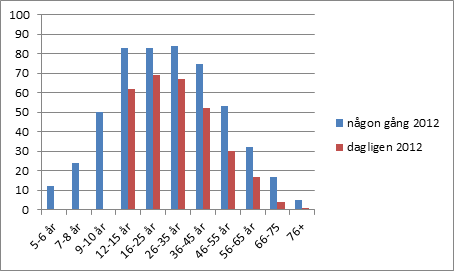
\includegraphics[scale=0.8]{pics/statistikalder.png}
    \caption{Andel procent av befolkningen som använder sig utav mobilt internet, statistik visar att den stora målgruppen är mellan 12-45 år gamla([s. 24]\cite{.se}).}
\end{figure}

\paragraph{Kontext}\mbox{}

Med kontext menas sidans typiska innehåll, det vill säga huvudsyftet med webbsidan. Beroende på webbsidans kontext kan användarna finna det simplare att använda antingen desktop eller mobilt, eller helt enkelt den enheten närmast till hands. Av de vetenskapliga artiklar som har tagits med i litteraturstudien har alla gemensamt att mobilt internet används flitigt för:

\begin{itemize}
	\item{Sköta E-post}
	\item{Sociala Nätverk}
	\item{Kolla nyheter, väder}
	\item{Söka information}
\end{itemize}
\bigskip
Andel procent av användarna skiljer sig beroende på artikel, då antalet användare för studien har varit olika, men visar ändå vad fokus läggs på när mobilt internet används. I Sverige uppskattas att 50 \% använder mobilt internet för att sköta e-post, 43 \% för socialt nätverk, 40 \% för att kolla vädret, nyheter och 18 \% för att söka fakta(\cite{.se}), i en daglig basis. I en annan studie där användningen utav mobilt internet analyserades med hjälp utav 109 deltagare visades sig att 70 \% av deltagarna använde mobilt internet för att kolla nyheter, väder och söka fakta, 13 \% utav deltagarna använde mobilt internet till sociala nätverk och 17 \% för att kolla på film och lyssna på musik(\cite{usageusability2}). I en liknande studie där istället 18 aktiva mobilanvändare studerades varje dag under en 4 veckors period, bestod den dagliga användningen av mobilt internet av 27 \% sociala nätverk, 24 \% koll på nyheter och vädret, 18.8 \% för email, 14.9 för vanligt surf, 10 \% för mobilt sök och 5.1 \% för kartor(\cite{mobilewebsearch}).

Vid desktop anses dessa fyra områden vara minst lika populär. I en studie som gjorde hos The Harris Polls Research(\cite{harrispoll}) samlades 2400 vuxna varav 991 mobilt internet användare för att se hur enheterna används i jämförelse beroende på kontext. I studien hamnade tre längst upp som de typer av hemsida vars desktopanvändare är ungefär lika stora om mobilanvändare.
\\
\begin{table}[H]
	\centering
	\begin{tabular}{|p{4cm}|p{4cm}|p{4cm}|}
	\hline
	~&Dator(desktop/laptop)&Mobil(Smartphone)\\ \hline
	Sköta E-post &90 \%&72 \%\\ \hline
	Sociala Nätverk&69 \%&64 \%\\ \hline
	Söka information&81 \%&45 \%\\ \hline
	*Kolla nyheter, väder&44.2 \%&52.1 \%\\ \hline
	\end{tabular}
    \caption {Områden i webben där användarna utnyttjar både mobil och desktop.}
\end{table}
\textit{*I studien ingick inte läsning utav nyheter, men i Q1 Research report för nyhetsläsning(\cite{q1research}) visades det sig, med undantag från målgruppen 65+, att majoriteten utav läsarna(59 \% till 77 \% i varje målgrupp) använder både mobil och desktop. Studien visar även att nyhetsläsare från mobilen numera är större än läsarna från desktop.}

I The HarrisPole Research fanns även siffror för områden där användaren föredrar en enhet mer än den andra.

\begin{table}[H]
	\centering
	\begin{tabular}{|p{4cm}|p{4cm}|p{4cm}|}
	\hline
	~&Dator(desktop/laptop)&Mobil(Smartphone)\\ \hline
	Fylla enkäter &86 \%&24 \%\\ \hline
	Handla produkter&78 \%&23 \%\\ \hline
	Navigation/Kartor&56 \%&73 \%\\ \hline
	\end{tabular}
    \caption {Områden i webben där användarna utnyttjar en enhet mer än de andra.}
\end{table}

\paragraph{Miljö} \mbox{}

En användares miljö har förändras tack vare mobilens storlek, det har gjort att miljön inte är längre är den vanliga sederliga hemma eller på kontor, utan kan vara i vilket sammanhang som helst och även vart som helst. Ett vanligt antagande är att mobilen endast används vid rörliga situationer(\cite[s.12]{mobilefirstluke}). Vilket vetenskapliga artiklar och statistik som har visar annat tvärtemot(\cite{mobilewebsearch}, \cite{mobilefirstluke}).

Författaren utav mobile first hänvisar(\cite[s.12]{mobilefirstluke}) till en enkätundersökning vilket visar användningen utav internet genom smartphones:
\begin{itemize}
	\item{84 \% använder det hemma}
	\item{80 \% använder det under diversa dödtid genom dagen}
	\item{74 \% använder det i kötid och väntan på möten}
	\item{69 \% använder det under shopping}
	\item{64 \% använder det på jobbet}
	\item{62 \% använder det medan man kollar på TV}
	\item{47 \% under pendling}
\end{itemize}
\bigskip

Att en stor andel av smartphonebärare använder sig utav mobilt internet i hemmet styrks utav fler vetenskapliga artiklar(\cite{mobilewebsearch}, \cite{mobilefirstluke}). Där orsakerna pekar åt bekvämligheten av att använda mobilen istället för datorn. Mobilen tillåter 1 minuts användning utav internet, t.ex. vid brådskande tillfällen, vilket kan anses vara omständliga via en desktop(\cite{mobilewebsearch}). I studien där 18 deltagare skulle föra dagböcker(\cite{mobilewebsearch}) under en period av 4 veckor var över 70 \% av inläggen om aktiviteter gjorda vid ett stationärt perspektiv, det vill säga antingen på jobbet eller i hemmet. Bara 17 \% av inläggen handlade om aktiviteter som gjordes vid resor, aktiviteter utomhus och vi pendling.
\\
\begin{itemize}
	\item{49,6 \% av inläggen handlade om aktiviteter gjorda i hemmet}
	\item{21,8 \% av inläggen handlade om aktiviteter på jobbet/universitetet}
	\item{11,4 \% av inläggen handlade om aktiviteter gjorda inomhus}
	\item{9,6 \% av inläggen handlade om aktiviteter gjorda under pendling eller transit}
	\item{7,2 \% av inläggen handlade om aktiviteter gjorda utomhus}
	\item{0,5 \% av inläggen handlade om aktiviteter gjorda under resa utomlands}
\end{itemize}
\bigskip

\subsection{Implementation}
\subsubsection{Prototyp}
Efter resultatet av litteraturstudien blev prototypen till webbsidan en nyhetssida. Grunden till valet gjordes med hänvisning till resultatet från litteraturstudien där statistik visar att andelen desktop och mobilbesökare hos en nyhetssida är jämnt fördelat, och även en av de största inom mobilområdet. För att skapa sidan gjordes en jämförelse mellan stora nyhetssidor så som aftonbladet.se, metro.co.uk, globalnews.ca, time.com, för att upprätthålla typiska element som finns i nyhetssidor. Allt som finns i ena vyn finns även i den andra.

\paragraph{Banner}\mbox{}

Banner visar tydligt vilken sidan man har kommit till. Beskriver namnet på sidan och en slogan som beskriver typen av webbsidan. Både i mobilt och i desktop går dessa inte att undgå, för att märka sig hos användaren, men är på mobilsidan mindre proportionerligt till artiklarna, tillskillnad från desktopvyn(\textit{figur 5}), för att undvika att bannern tar för stor plats på mobilskärmen(\textit{figur 6}).
\\
\begin{figure}[H]
\centerline{%
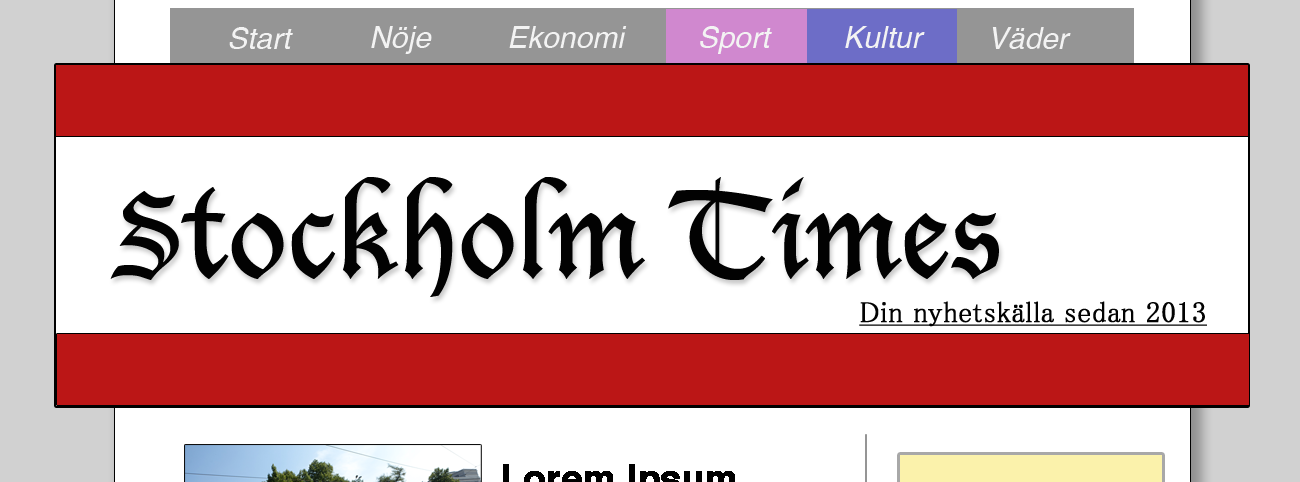
\includegraphics[scale=0.258]{pics/bannerdesktop.png}\hspace{2em}%

\includegraphics[scale=0.40]{pics/bannermobil.png}%
}
\vspace{0.3cm}
\hspace{0.15cm}Figur 5: Banner för desktopvyn.\hspace{4.4cm} Figur 6: Banner för mobilvyn.

\end{figure}

\paragraph{Menyer}\mbox{}

Nyhetssidorna som granskades hade alla minst tre olika sorters menyer, en huvudmeny, en mindre meny bestående av typiska ”skapa konto, logga in” länkar(\textit{figur 7}), samt en nedre meny längst ner på sidan med diverse länkar(\textit{figur 9}). I mobilvyn, behölls nedersta menyn, men de två översta sattes ihop och gömdes under en meny knapp för att spara plats på mobilskärmen(\textit{figur 8}).
\\

\begin{figure}[H]
\centerline{%
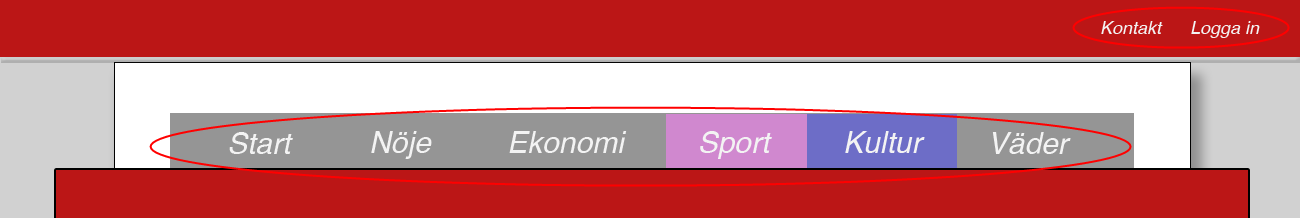
\includegraphics[scale=0.4]{pics/menydesktop.png}\\
}
\end{figure}
\hspace{0.5cm}Figur 7: Huvudmenyn i desktopvy.

\begin{figure}[H]
\centerline{%

\includegraphics[scale=0.6]{pics/menymobil.png}\hspace{2em}%
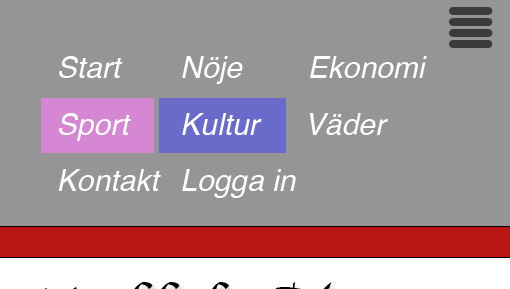
\includegraphics[scale=0.35]{pics/menymobilopen.png}%
}
\end{figure}
\hspace{0.5cm}Figur 8: Huvudmenyn i mobilvyn.

\begin{figure}[H]
\centerline{%
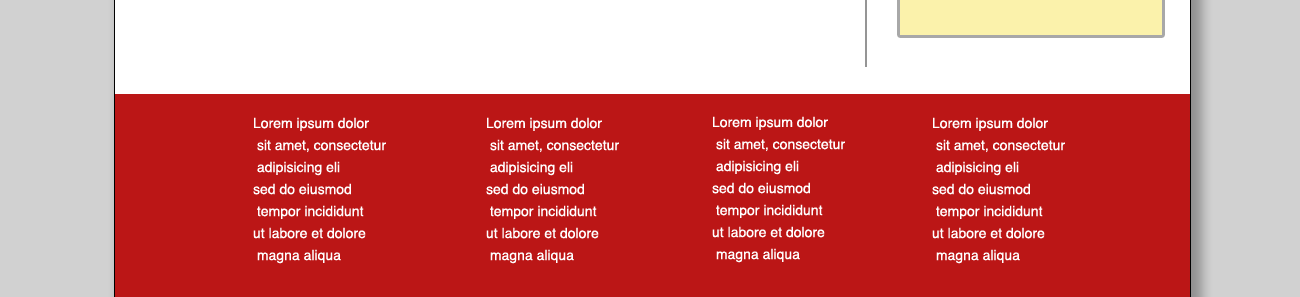
\includegraphics[scale=0.237]{pics/menydesktopbot.png}\hspace{2em}%
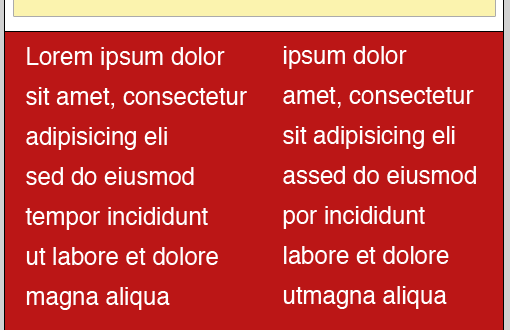
\includegraphics[scale=0.35]{pics/menymobilbot.png}%
}
\end{figure}
\hspace{0.5cm}Figur 9: Nedremenyn i desktopvyn och mobilvyn.
\newpage
\paragraph{Artiklar och Annonser}\mbox{}

För artiklarna och annonserna, prioriterades dessa ungefär lika högt i desktopvyn(\textit{figur 10}), mestadels för att annonser anser vara en viktig faktor till nyhetssidors intäkter nu när nyhetssidor kan ses på webben. Dessvärre inte lika hög prioriterat i mobilläge då det finns mindre yta och artiklarna är huvudelementen i nyhetssidan, därför hamnar annonserna efter artiklarna(\textit{figur 11}). Artiklarna har alla samma storlek men skiftar i plats på bild och text, för att skapa en mer levande känsla när man ser webbsidan. Annonsernas design härstammar från aftonbladet.se, där färgen på bakgrunden samt texten får läsaren att förstå att det är annonser. 
\\

\begin{figure}[H]
\centerline{%
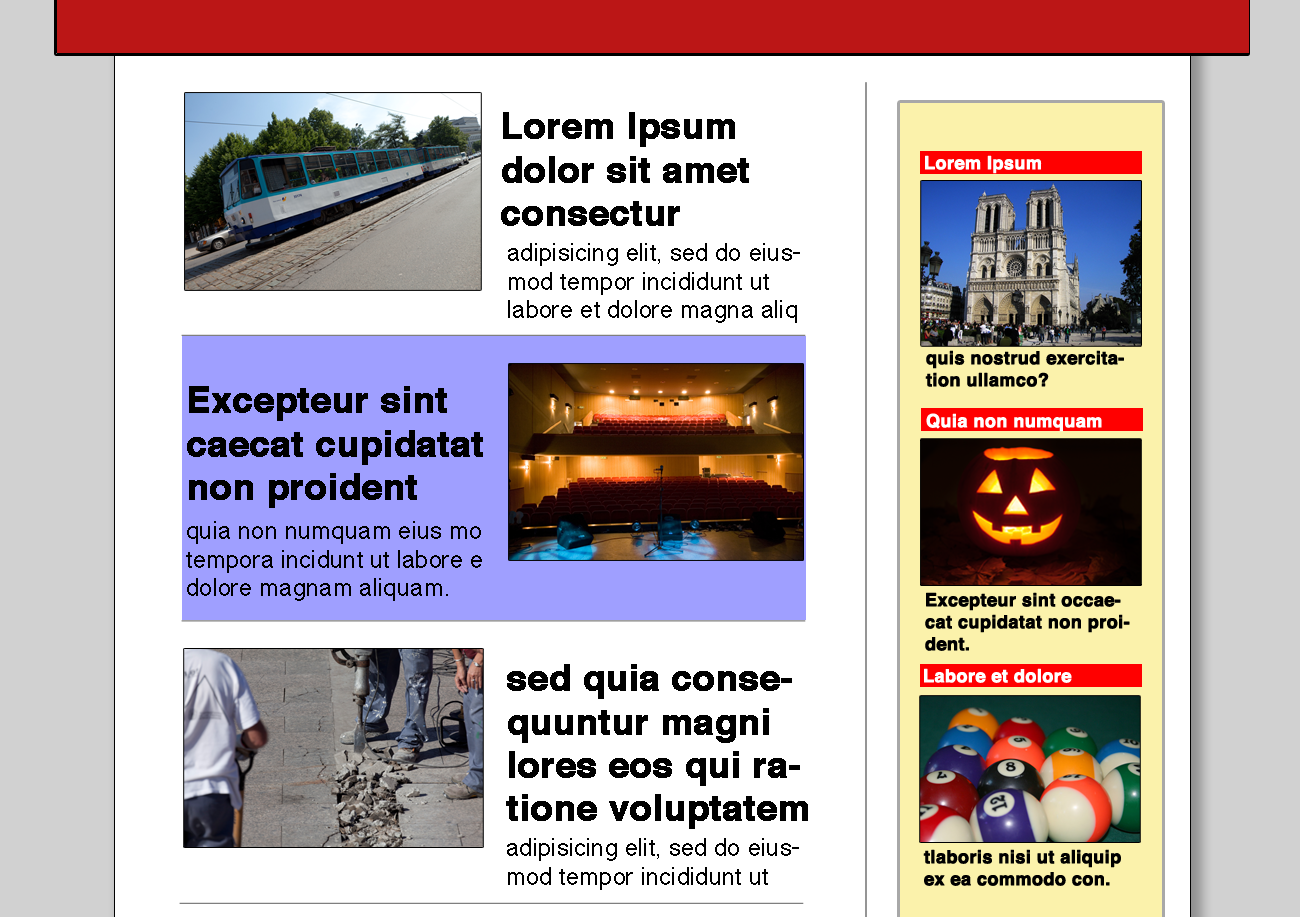
\includegraphics[scale=0.3]{pics/artikelannonsdesktop.png}
}
\end{figure}
\hspace{0.5cm}Figur 10: Artiklar och annonser i desktopvyn.
\\
\begin{figure}[H]
\centerline{%
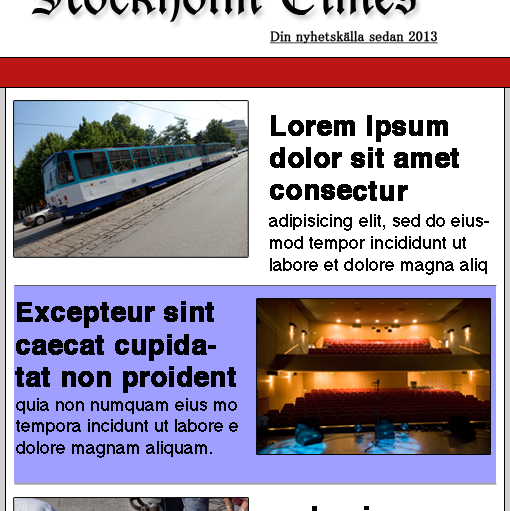
\includegraphics[scale=0.35]{pics/artikelmobil.png}\hspace{2em}%
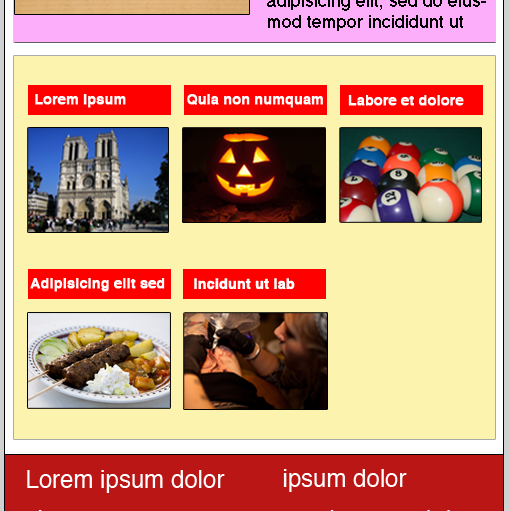
\includegraphics[scale=0.35]{pics/annonsmobil.png}%
}
\end{figure}
\hspace{0.5cm}Figur 11: Artiklar och annonser och mobilvyn.

\paragraph{Färgmarkeringar}\mbox{}

Färgmarkeringen görs i webbsidan för att markera olika typer av artiklar, i nyhetssidor görs detta normalt för att markera artiklar som tillhör en annan sektion av tidningen, så som sport, ekonomi, kultur osv. I prototypen markeras sport och kultur med en rosa och blå färg vilken även blir färgen för respektive länk(\textit{figur 12}).
\\

\begin{figure}[H]
\centerline{%
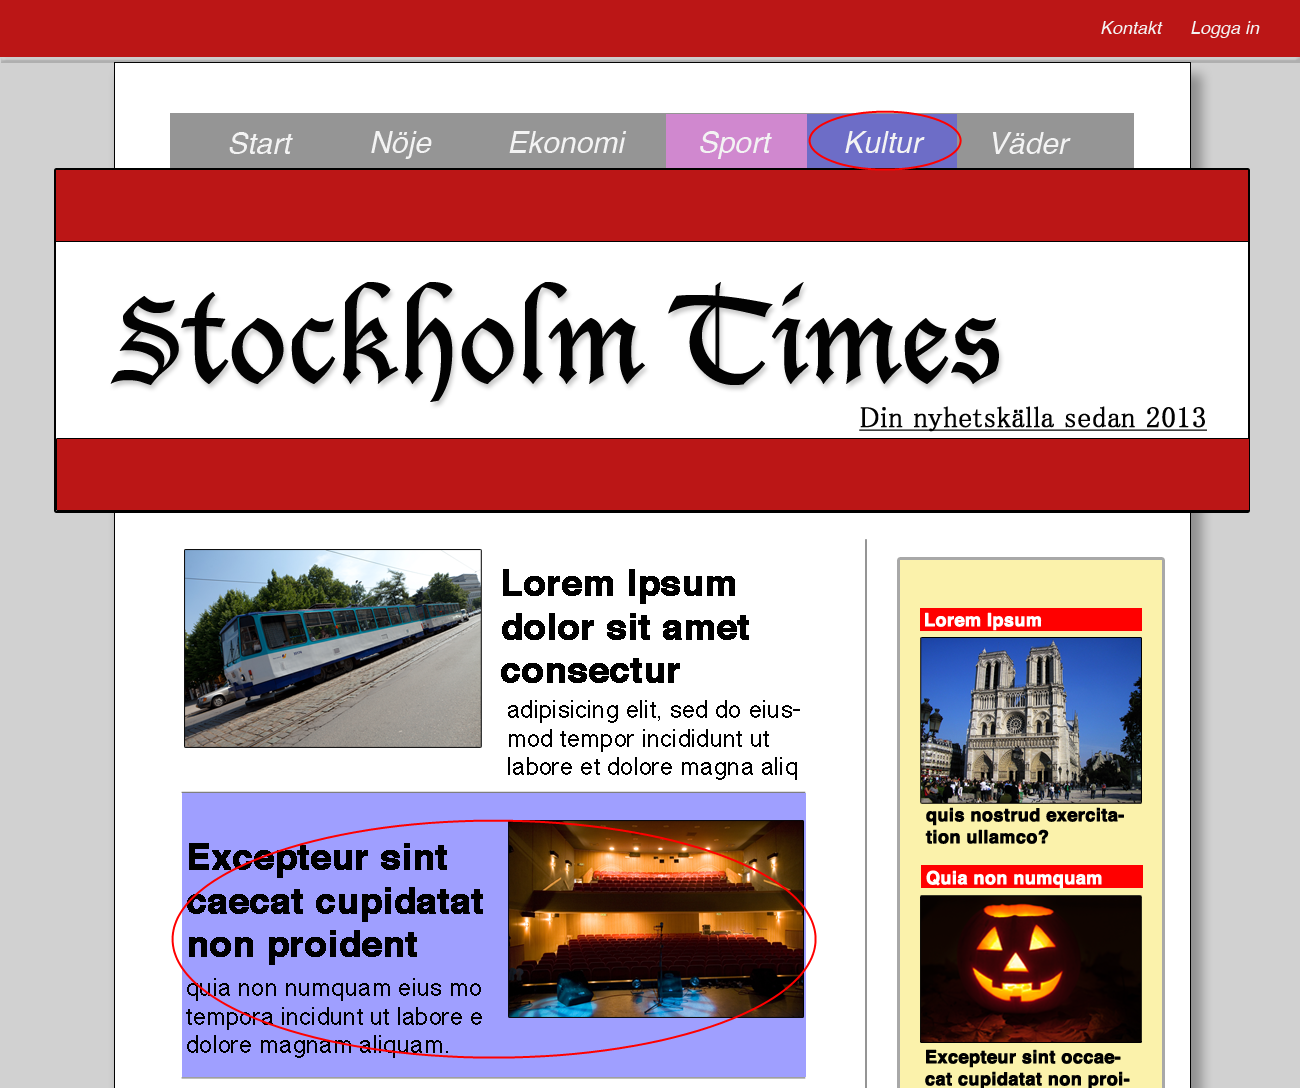
\includegraphics[scale=0.25]{pics/fargdesktop.png}\hspace{2em}%
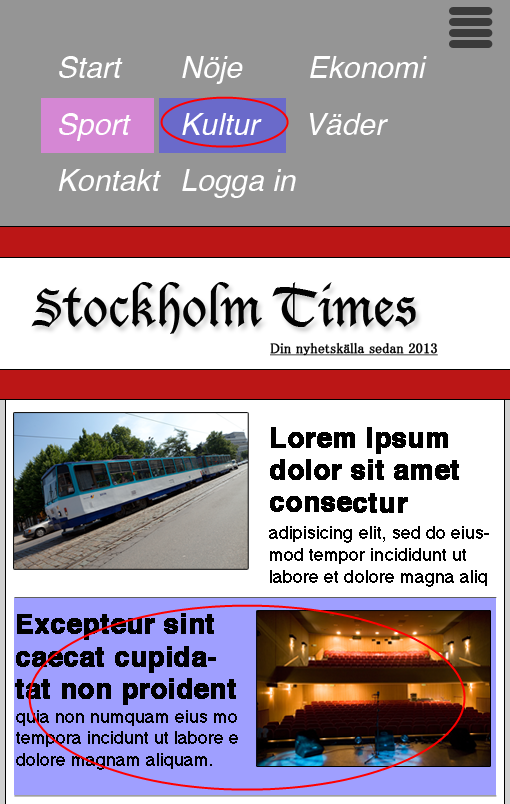
\includegraphics[scale=0.3]{pics/fargmobil.png}%
}
\end{figure}
\hspace{0.5cm}Figur 12: Lilla/blå färgmarkering för kultursektionen.


\subsubsection{Responstid}

Nedan visas tre olika hämtningar av bägge webbsidor, både i desktopmiljö samt mobilmiljö. Värdena som har antecknats är responstiden för hämtning av HTML-filen samt CSS-filen. T.ex I mobile-first tog det 19ms för att hämta mobilsidans css-fil, i desktop-first tog det längre tid, 36ms. Däremot tog mobile-first 23ms att hämta desktopsidans css-fil, vilket gick snabbare i desktop-first, då det tog 21ms. De tre olika hämtningar visar relativt lika siffor vilket betyder att hämtningar från mobilsidan görs snabbare i mobile-first än desktop-first. Hämtningar från desktopsidan görs däremot snabbare med desktop-first.
\newpage
\textbf{Hämtning 1}

\begin{table}[H]
	\centering
	\begin{tabular}{|p{2.5cm}|p{2.7cm}|p{2.4cm}|p{3.1cm}|p{2.8cm}|}
	\hline
	~&\textbf{.html mobilvy}&\textbf{.css mobilvy}&\textbf{.html desktopvy}&\textbf{.css desktopvy}\\ \hline
	\textbf{Desktop-first}&73ms&36ms&36ms&21ms\\ \hline
	\textbf{Mobile-first}&36ms&19ms&39ms&23ms \\ \hline
	~&~&~ &~&~\\ \hline
	\end{tabular}
    \caption {Värden från första hämtningen av prototypsidan.}
\end{table}

\textbf{Hämtning 2}

\begin{table}[H]
	\centering
	\begin{tabular}{|p{2.5cm}|p{2.7cm}|p{2.4cm}|p{3.1cm}|p{2.8cm}|}
	\hline
	~&\textbf{.html mobilvy}&\textbf{.css mobilvy}&\textbf{.html desktopvy}&\textbf{.css desktopvy}\\ \hline
	\textbf{Desktop-first}&19ms&22ms&46ms&20ms\\ \hline
	\textbf{Mobile-first}&33ms&20ms&22ms&22ms \\ \hline
	~&~&~ &~&~\\ \hline
	\end{tabular}
    \caption {Värden från andra hämtningen av prototypsidan.}
\end{table}

\textbf{Hämtning 3}

\begin{table}[H]
	\centering
	\begin{tabular}{|p{2.5cm}|p{2.7cm}|p{2.4cm}|p{3.1cm}|p{2.8cm}|}
	\hline
	~&\textbf{.html mobilvy}&\textbf{.css mobilvy}&\textbf{.html desktopvy}&\textbf{.css desktopvy}\\ \hline
	\textbf{Desktop-first}&73ms&36ms&36ms&21ms\\ \hline
	\textbf{Mobile-first}&36ms&19ms&39ms&23ms \\ \hline
	~&~&~ &~&~\\ \hline
	\end{tabular}
    \caption {Värden för tredje hämtningen av prototypsidan.}
\end{table}


\subsubsection{Kodstorlek}

Tabellen visar storleken på css-filen i både antal rader och filstorlek. Den visar att CSSen för mobil-first är större än CSSen för desktop-first i filstorlek. Däremot har den i desktop-first fler rader än den i mobile-first. I mobile-first CSSen är uppdelningen mellan rader i grundkod och rader i media queries 193 mot 180. I den för desktop-first består största delen utav rader i grundkoden, där är uppdelningen 221 mot 160.

\begin{table}[H]
	\centering
	\begin{tabular}{|p{6cm}|p{2.7cm}|p{2.4cm}|}
	\hline
	\textbf{main.css}&\textbf{Desktop-first}&\textbf{Mobile-first}\\ \hline
	\textbf{Antal rader i grundkod}&221st&193st\\ \hline
	\textbf{Antal rader i media queries}&160st&180st\\ \hline
	\textbf{Totalt antal rader}&381st&374st\\ \hline
	\textbf{Filstorlek}&5.2kb&5.6kb\\ \hline
	\end{tabular}
    \caption {Värden från main.css.}
\end{table}

\subsubsection{Implementeringstid}

Implementeringstiden redovisas utifrån dagboken som skrevs under implementeringstiden. I resultatet visar skillnaden mellan implementeringstiden för grundsidan och tiden som krävdes för att göra webbsidan responsivt. I mobile-first tog grundsidan mindre tid att implementera än att göra webbsidan responsiv, i desktop-first tog det däremot längre tid att implementera grundsidan. Desktop-first tog totalt längre tid att implementera än mobile-first. Ta i beaktande att implementeringen gjordes utav en junior inom området gränssnittsutveckling, samt att desktop-first implementerades före mobile-first.

\begin{table}[H]
	\centering
	\begin{tabular}{|p{6cm}|p{2.7cm}|p{2.4cm}|}
	\hline
	~&\textbf{Desktop-first}&\textbf{Mobile-first}\\ \hline
	\textbf{Tid för grundsidan}&14.5h&6.5h\\ \hline
	\textbf{Tid för responsive}&7.5h&10h\\ \hline
	\textbf{Totalt antal rader}&22h&16.5h\\ \hline
	\end{tabular}
    \caption {Värden på implementationstid, tagna från dagboken.}
\end{table}

\subsubsection{Kommentarer från dagboken}

\textbf{Desktop-first}
\\\\
\textit{”Mycket småpill i början, många element att finslipa, göra fina och sätta på plats.”}\\\\
\textit{”Oerhört lätt att göras till responsive så länge man har använt sig av fluid grid och fluid layout från början. Allt renderas av sig självt och så fort det ser konstigt ut, modifieras CSSen i en media querie.”}\\\\
\textit{”Lång tid i början, i jämförelse med responsive delen, förvånad över att responsivedelen gick så smidigt. Endast lite småpill lite här och där för att. Det mesta hade fixats under desktoputseendet.”}\\\\
\textit{”Inte så många media queries, sidan ser bra ut mellan media queries. Mycket kod i grunden som är avsedd för desktop, inte lika mycket i media queries.”}\\\\
\\
\textbf{Mobile-first}
\\\\
\textit{”Enkelt att påbörja med, följer skissen uppifrån neråt, går inte att tappat bort sig åt kanterna utan elementen är så pass små att det känns som att de finns i en smal led att följa.”}\\\\
\textit{”Behövs mycket småpill mellan media queries, media queries kommer i början hyfsat tät inpå varandra enbart för att fixa små fel som margins och padding så att elementen håller sig på ett och samma ställe. Samt för förstoring av text, så det är väldigt litet i början och måste förstoras relativt till andra element.”}\\\\
\textit{”Gäller att hitta en struktur redan från början mellan skisserna, blir en några refaktoreringar för att få webbsidan då bredden är 768px att se perfekt ut, eftersom mycket kommer just under den vyn. Som att lägga vissa element i hållare”}\\\\
\textit{”Från 768px till desktop-size gick väldigt smidigt.”}\\\\
\textit{”Väldigt lätt i början, enkel struktur att lägga upp för mobilen, responsivt höll till 480px och till och med 768px var det mycket att fixa med hjälp av media queries, då många element går från att vara under varandra till att vara bredvid varandra.”}\\\\
\textit{”Viktigt att planera och lägga en struktur på hur den ska övergå till desktop. Mycket kod i media queries sektionen, lite kod i grunden för mobilvyn.  Ser bra ut mellan mobilvyn och desktopvyn.”}\\\\
\section{Diskussion och Analys}
\printbibliography

\end{document}



